% Software Backend (Python)
% Zuständig: Jones

% wie/wo soll protobuf erklärt/erwähnt werden?

\chapter{Software - Backend}
\label{sec:software_backend}
\initials{JS}
Das Backend ist die zentrale Rechenstelle, 
welche in mehrere Komponenten aufgeteilt ist.
% generell zum backend

\begin{figure}[H]
    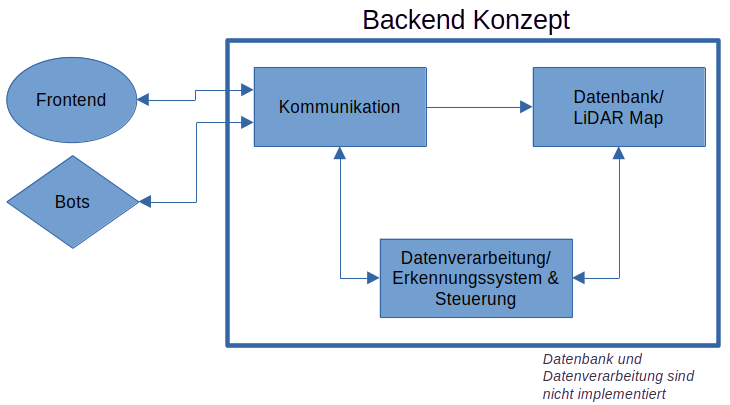
\includegraphics[width=\textwidth, center]{img/backend-konzept.png}
    \caption{Backend Konzept}
    \label{fig:backend_konzept}
\end{figure}
% grafik anpassen

Es ist verantwortlich für die Kommunikation und Datenerfassung 
zwischen allen Teilnehmern. 
Dazu gehören die drei Roboter, welche die Sensordaten liefern
und das Frontend, 
zu dem die Daten zur Visualisierung und Mitverfolgung gesendet werden.

Weiters findet hier die zentrale Datenverarbeitung und Verwaltung statt: 
Die Erstellung der LiDAR-Map, 
die Ermittlung der Roboterpositionen und gegebenenfalls die Berechnung der Messwerte. 
% im falle ineffizient etc
Eine weitere Aufgabe des Backends 
ist die Steuerung der Roboter mithilfe eines Erkennungssystems, 
welches nach bestimmten Kennzeichen in den erhaltenen Daten Ausschau hält 
und damit die einzelnen Bots erkennt und verfolgt, 
um deren Positionen relativ zur LiDAR-Map ausfindig zu machen.
% 
% Die Zentrale Datenverarbeitung und autonome Steuerung der Roboter sind 
% im zu zeitigen Prototypen stand nicht implementiert.
% % stattdessen weiterleitung und fernsteuerung
% TODO 

Letztendlich verwaltet das Backend die Datenbank, 
welche die etwaigen Daten der Datenverarbeitung und des Erkennungssystems speichert.
%
Insbesonders relevant ist hierzu die LiDAR-Map.
%
Für die Programmierung des Backends wurde die Sprache Python gewählt, 
welche mit ihrer Vielzahl an Standard- und externen Paketen 
und Frameworks eine effiziente und schnelle Programmierung unterstützt.
%
Danke der aktiven Python-Community gibt es auch online sehr viele Foren,
in denen man Unterstützung findet.
% 
Für dieses Projekt wurde es aufgrund seiner Vielseitigkeit gewählt, 
speziell in Bezug auf die unterschiedlichen Tasks, 
die ausgeführt werden müssen, 
hauptsächlich in Bezug auf Kommunikation und Datenverarbeitung, 
in denen Python üblicherweise verwendet wird.
% 
Dabei müssen auch mehrere WebSocket-Verbindungen offen bleiben und verwaltet werden. 
Anhand dieser wesentlichen Vorraussetzungen wurde ein Serverkonzept definiert, 
welches schnell mithilfe von Paketen realisiert wurde. 
%
Effiziente und strukturierte Programmierung und Modifizierung ist wesentlich, 
weil der Backend-Code kontinuierlich wächst.
% 
Dies wurde auch durch Erfahrungen mit dem Vorgänger-Projekt untermauert --
ein wesentlicher Teil davon bestand aus der Kommunikation über Websockets.
% Gelaber über python
% wegen math Funktionen...
% schnelle Modifizierung 
% packet/ Bibliothek Fokussierung auf Einfachheit
\section{Systembeschreibung}
\initials{JS}
% drunter verschoben weil besseres layout?
In diesem Abschnitt wird genauer 
über die geplanten einzelnen Komponenten 
und deren Funktion gesprochen.
%
Zu beachten ist, dass nicht alle geplanten Systeme, die hier beschrieben sind, 
implementiert wurden und manche noch in der Konzeptphase sind.
Für den tatsächlichen Stand siehe Abschnitt \ref{subsec:backend_aktueller_stand}.
%
\subsection{Datenverwaltung}
\label{subsec:backend_data}
\initials{JS}
% übersicht über die drei komponenten und wie ungefähr der datenfluss aussieht?
% TODO
% Datenbank für lidar?
% TODO

% TODO bevor abgabe
% womöglich löschen
Dieser Abschnitt bespricht kurz den Datenablauf 
zwischen den Teilnehmern und den internen Komponenten.
% 
Weil Teile des Backends nicht realisiert sind,
konnte die Datenverarbeitung ebenfalls noch nicht aufgebaut werden,
weswegen hierzu nicht viel gesagt werden kann.

\subsection{Kommunikation}
\label{subsec:Kommunikation}
\initials{JS}
Die drei Roboter sind aktive Teilnehmer in der Kommunikation, 
das heißt, die Verbindung ist permanent aufrechtzuerhalten, 
bidirektional und zeitlich synchronisiert. 

Zur Verbindung entschieden wir uns für das Kommunikations-Protokoll WebSocket.
% 
Dieses ermöglicht eine Verbindung zwischen Client und Server,
welche im Vergleich zu gewöhnlichen HTTP-Anfragen offen bleibt, 
wodurch bidirektionale Echtzeitkommunikation möglich ist.
% könnte man mehr ausschreiben aber schau ma später

\subsection{Datenverarbeitung}
\initials{JS}
% TODO
Eine Aufgabe des Servers ist die Verarbeitung der erhaltenen Daten, 
sowie die Weiterleitung zum Frontend.
% 
Um große Belastungen durch die Auswertung von Sensordaten auf den Robotern zu vermeiden, 
werden einige Arbeiten auf den Server ausgelagert.
%
Außerdem stehen in Python bereits ausgebaute Mathematik-Pakete zur Verfügung,
welche Verwendet werden können,
um die Sensordaten zu interpretieren. 
%
Ebenso gibt es Softwarepakete zur Datenanalyse und -manipulation.

\subsection{Erkennungssystem}
\initials{JS}
Geplant war,
dass aus den erhaltenen Daten mit der Zeit eine Karte erstellt wird, 
sozusagen die LiDAR-Map, 
welche in einer Datenbank abgespeichert wird.
% 
Über die Zeit werden Datenpunkte gesammelt, 
die sich nach einem gewissen Muster sammeln 
und ein klareres Bild über die Form eines Raumes geben.
%
Diese Muster, z.B. gerade Linien und Ecken,
werden vom System erkannt.
Anhand dieser daten wird dannn ermittelt, 
wo ungefähr sich die Roboter befinden.
%
Dies wird mit einem weiteren Erkennungssystem für Tamerlan \& Bambi kombiniert, 
welches zuständig ist,
die Position der beiden zu ermitteln,
indem auf den Bots identifizierbare reflektieren Objekte befestigt werden, 
beispielsweise Zylinder, wodurch sie erkannt werden können.
%
Mit diesen Informationen kann die autonome Fernsteuerung der Roboter folgen.
% füge skizzen hier oder erklär anderen Kapitel?
% Kugel, stab, mehrere stäbe, reflektierendes material

Eine genauere Beschreibung der LiDAR-Karte und wie diese aussieht, 
ist im Abschnitt \ref{subsec:frontend_lidar_map} 
auf Seite \pageref{subsec:frontend_lidar_map} zu finden.

\subsection{Steuerung der Roboter}
\label{subsec:backend_robot_detection}
\initials{JS}
% TODO
Zurzeit nicht realisiert.
% spätester schritt weil funktionierende Strategie benötigt wird zur Erkennung
% Datenbank/ Datenbearbeitung

Die Aufträge der einzelnen Bots 
sind in den entsprechenden Kapiteln genauer beschrieben.
% schau was da steht und was speziell hier klargemacht werden muss

Es sind zwei Steuerungen geplant:
die manuelle Steuerung und die automatisierte.
% 
Die manuelle Steuerung geschieht über das Frontend, 
womit man die Roboter mithilfe der Visualisierungen 
und der Videoübertragung steuern kann.
% 
Die automatisierte Steuerung geschieht mithilfe des Erkennungssystems 
und soll den Bots erlauben,
mithilfer der erstellten LiDAR-Karte zu navigieren. 
Dadurch sollen die beiden blinden Bots (Tamerlan \& Bambi) dem Guide folgen.
% verwendung von code vom vorgänger Projekt

\section{Aktueller Stand}
\label{subsec:backend_aktueller_stand}
\initials{JS}

\begin{figure}[H]
    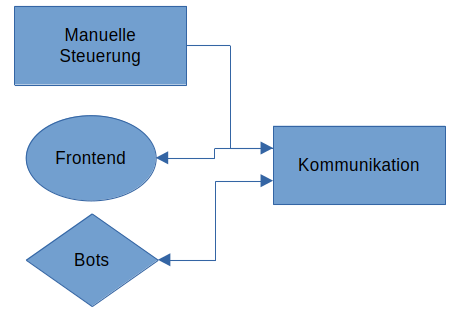
\includegraphics[width=0.7\textwidth, center]{img/Backend/backend-aktuell.png}
    \caption{Backend Aktuell}
    \label{fig:backend_konzept}
\end{figure}

% Womöglich Teile zu Ergebnisse verschieben?
Zum Zeitpunkt der Abgabe dieser Diplomarbeitsabgabe 
sind nicht alle geplanten Features für das Backend implementiert.
%
Für erste Tests wurde der Kommunikationsteil so realisiert, 
dass dieser als ``Weitergabe'' fungiert.
%
Dies wurde so realisiert,
dass die Daten zwischen einem Bot und dem Server weitergegeben werden,
quasi wie ein Router.
%
Der nächste Schritt besteht dann,
über eine Prototyp Steuerung Befehle zu den einzelnen Bots zu senden.
%
Der Prototyp für die Steuerung ist als manuelle Steuerung realisiert. 
Der gewählte Roboter wird manuell von einem Nutzer bedient.
%
In Zukunft kann die manuelle Steuerung als eine weitere Option beibehalten werden, 
die die automatisierte Steuerung überschreiben kann.
%
Dies kann verwendet werden, 
um beispielsweise den Guide manuell in bestimmte Bereiche zu führen,
oder um bestimmte Features zu testen.

\section{Backend - Code}
\initials{JS}
In diesem Abschnitt wird genauer auf den Code des Backend Prototyps
und dessen technische Realisierung eingegangen. 
%
Weiters wird auch beschrieben,
welche Pakete und Werkzeuge verwendet wurden. 

\subsection{Zusätzlich verwendete Tools und Workflow}
\initials{JS}
% algemein zu python workflow
% womöglich unötig
% TODO
\subsubsection{Formatter und Linter} 
\initials{JS}
Um gute Lesbarkeit zu gewährleisten, 
ist eine ordentliche Struktur und Formatierung in jedem Code notwendig.
%
Es ist schwierig, eine gute Konsistenz beizubehalten, 
weshalb heutzutage fast immer Formatierungstools und Linters verwendet werden. 
%
Linters sind Programme, welche automatisch den Code überprüfen, 
um stilistische Fehler und Einhaltung von Code-Standards sicherzustellen.
%
Dies soll helfen,
die Code-Qualität zu verbessern 
und eventuelle Fehler frühzeitig zu erkennen.
%
Die Standard-Erweiterung für Python von Visual Studio Code 
beinhaltet kein Formatierungstool.
%
Dafür wurde der Formatter \texttt{autopep8} verwendet, 
weil er die Eigenschaft hat,
den Originalstil des Schreibers beizubehalten
und nur Änderungen für die Lesbarkeit durchzuführen. 
%
Dazu passend ist der Linter \texttt{Flake8},
welcher standardmäßig 
dem gleichen Styleguide \text{PEP 8} folgt.
% weil vscode es standart mäßig Formatierung nicht mitliefert
% \subsubsection{venv/environment management}
% \initials{JS}
% % TODO
% Falls sich nicht viel ändert, ist dieser Abschnitt wahrscheinlich nicht nötig, 
% da nicht viel besonders ist.


\subsection{Python Packages}
\initials{JS}
% TODO schau dir dieses abschniit nochmal durch
Um gegebene Funktionen zu gewährleisten,
sind weitere externe Pakete nötig, 
die nicht Teil der Standardumgebung sind.
%
Welche aktuell verwendet werden,
ist in diesem Abschnitt erklärt.

\subsubsection{websockets}
\initials{JS}
Für Python ist ein WebSocket-Paket namens 'websockets' vorhanden, 
welches die Client-Server Kommunikation um ein Vielfaches vereinfacht, 
da man sich keine Sorge über Handshakes, Ping Pongs, 
oder anderes Verhalten der Websocket Spezifikation machen muss.
%
Das gesamte WebSocket-Protokoll wird von dem Paket geregelt 
und man kann sich auf die Nutzdaten konzentrieren, die übertragen werden.
%
Es sind dennoch einige Parameter zur Verfügung gestellt, 
um das Verhalten zu modifizieren.
% code beispiele?

% erklärung zu den packet Webscoket
Die Standardimplementierung des verwendeten WebSocket-Pakets basiert auf \texttt{asyncio}.
%
\texttt{asyncio} ist die eingebaute Implementierung von Co-Routinen in Python,
welche das Schreiben von asynchronen Frameworks erlaubt.
% 
Ein weitverbreiteter Anwendungsfall von \texttt{asyncio} besteht in der interaktion mit Netzwerken,
da Netzwerkanfragen eine gewisse Zeit brauchen.
% snippet zu asyncio, könnte mehr schreiben?
Alternativ ist eine \texttt{threading}-Implementierung für WebSocket-Paket verfügbar. 
Für dieses Projekt wurde \texttt{asyncio} gewählt,
weil Thread-sicherer Code komplexer zu gestalten ist.
% warum nicht? kann später bei optimierungsmöglichkeiten erklärt werden
Eine Sans-I/O Implementierung ist auch vorhanden, 
jedoch für dieses Projekt zurzeit irrelevant.

\subsubsection{protobuf}
\initials{JS}
Das Besondere an der \texttt{protobuf} Implementierung hier in Python ist,
dass sehr viel von dem protobuf Paket selbst erledigt wird.
%
Im Vergleich zum Vorgängerprojekt,
wo die Datenpakete manuell in in Binärformat ``zusammengebaut'' werden mussten, 
wird mit der \texttt{protobuf} ein Objekt erstellt
und mittels einer Funktion automatisch in ein Binärformat zum Datentransfer umgewandelt.
% verhalten in python
% wie anders

% Kurzeitig gab es das Problem wie genau mit dem protobuf paket zu arbeiten ist,
% aufgrund dessen das die dokumentation nicht der von anderen Python Paketen gleicht
% und alle Informationen hauptsächlich von der Anleitungen zu Wünschen übrig lässt.
% Ich hatte einfach ein wenig probleme es anfänglich zu kapieren aber ging schnell

\subsubsection{pygame}
\initials{JS}
Dieses Paket wird ausschließlich für die manuelle Steuerung verwendet.
%
Hauptsächlich wird es zum Entwickeln von Spielen in Python genutzt,
doch in diesem Projekt dient es der einfachen Konfiguration von Spielcontrollern,
welche zur Steuerung verwendet werden.

\subsection{Kommunikation - test\_server\_passby.py}
\initials{JS}
In diesem Abschnitt wird über die Kommunikation 
und bestimmte technischen Implementierungen angesprochen.

Der Prototyp hat die Funktion, zwei Typen von Verbindungen zu bearbeiten: \\
%
1. Die der Bots, welche als Server agieren; 
das bedeutet, 
dass sich dieser Backend-Server mit den drei Robotern verbinden muss, 
während das Frontend standardmäßig als Client fungiert. 
Das heißt, dass die Clients eine Verbindung mit dem Backend Server herstellen. \\
% 
2. Die Verbindung mit dem Frontend, 
welche vom Server für einkommende Verbindungen bereitgestellt werden muss.
% 
Die Daten, die von der jeweiligen Seite kommen, 
werden zurzeit zur anderen Stelle weitergeleitet.

Dementsprechend ist die Kommunikation auf zwei Tasks aufgeteilt,
die des Frontends und die der Roboter.
% 
Beide Tasks starten einen weiteren Subtask, welcher nebenbei laufen wird, 
dieser hat entsprechend die Aufgabe, 
solange die Websocket Verbindung offen ist,
die ankommenden Pakete zu erwarten 
und diese entsprechend in einen Puffer abzulegen, 
um weiter verarbeitet zu werden. 

Beide Tasks verarbeiten die Queues, 
in denen eine bestimmte Anzahl der Elemente im Puffer 
einzeln geholt und die Protobuf Wrapper verarbeitet werden.
% 
Im derzeitigen Prototyp werden die Daten in die Konsole ausgegeben,
und zur Sendung der Gegenseite in eine weitere Queue 
für einen beliebigen Roboter bereitgestellt, 
oder im Code des derzeitigen Roboter-Handler 
an alle verbundenen Frontends gesendet.
% 
Dies ist eine Vorbereitung auf die nächsten Iterationen 
(Weitergabe in die Datenbank und Datenverarbeitung).

% übersichtsgrafik über teilnehmer und wie datenablauf funktioniert
% asyncio - warum
% main task überblick (server und drei clients) warum so aufgeteilt?
% subtask

\subsubsection{asyncio}
\initials{JS}
% erklärung zu asyncio
Um mehrere separate Tasks auszuführen, wurde asyncio,
die eingebaute Implementierung von Koroutinen in Python, verwendet.
% 
Asyncio funktioniert, 
indem Tasks sich die gleiche CPU-Zeit mittels einem Event-Loop teilen.
%
Dies geschieht, indem sie mit dem 'await' Befehl freiwillig die Kontrolle abgeben,
wenn sie auf etwas warten (z.B. dass Daten vom Websocket ankommen).
%
Währenddessen wird der Event-Loop andere Tasks durchführen, 
solange der erste Task wartet.
%
Im Gegensatz zu üblichem Multitasking,
wo jeder Task eine feste Zeit vom Betriebssystem zugeschrieben bekommt, 
und es entscheidet, wenn ein Task an der Reihe ist.
% 
Der größte Unterschied jedoch ist das \texttt{asyncio} Tasks sich alle einen Thread teilen.
%
Dies bedeutet das Asyncio Programme nur einen einzelnen Kern verwenden.
% 
Da wir von der erhöhten Leistungsfähigkeit von Threading nicht wirklich profitieren
(weil wir nur vier Teilnehmer haben),
haben wir uns für die Effizienz und Skalierbarkeit von \texttt{asyncio} entschieden.

% TODO Womöglich weiter beschreiben, wie asyncio genau funktioniert?
% Frag ob das so passt jetzt?

\subsubsection{Queue Buffers}
\initials{JS}
% FIFO Queues
% Wichtigkeit nicht blockierendes verhalten um asynchrones workflow zu gewährleisten
Damit keine Nachrichten verloren gehen, 
weil die adressierten Prozesse gerade nicht aktiv sind,  
wird der Empfang von Websockets von der Backend-Logik abgekoppelt.
%
Dafür werden Queues, welche als FIFO-Buffer realisiert wurden,
verwendet. Diese agieren als Zwischenspeicher, 
wo die erhaltenen Daten von den Websockets landen, 
um dann später weiterverarbeitet zu werden.
% 
Somit können wir einen Prozess starten, 
welcher auf eingehende Nachrichten warten kann,
während unser Backend andere Prozesse ausführt.
% kann mehr dazu schreiben
% ermöglicht auch sachen etc.
% TODO

\subsection{Prototyp manuelle Steuerung}
\initials{JS}
Die Steuerung soll einem Bediener erlauben,
manuell die Bots zu steuern. 
% 
Dafür verwenden wir einen PlayStation-Controller, 
weil wir bereits im Vorgängerprojekt
eine solche Steuerung realisiert haben.
%
Deshalb ist ein Großteil der Arbeit hier die Anpassung an das neue Datenformat, 
Verwendung neuer Websocket-Pakete und Modifizierung der Berechnungen.
% 
Dies wurde zuerst als einzelnes Skript zu realisiert, 
welches den Platz des Frontends einnimmt. 
Im Laufe des Projekts wurde dieses dann ins Frontend integriert und teilweise neu implementiert.

% TODO aktualisiere dies entsprechend
% TODO
\subsubsection{Controller Steuerung}
\initials{JS}
Dafür wird das Paket \texttt{pygame} verwendet,
das für die Verbindung mit den Controllern verantwortlich ist.
unabhängig davon, ob sie verkabelt oder über Bluetooth verbunden sind.
%
Dieses Paket funktioniert sowohl für Controller welche mit USB verbunden sind,
als auch für solche, die die Drahtlose Bluetooth-Schnittstelle nutzen.

\subsubsection{Begrenzung Änderungsrate}
\initials{JS}
Ein zusätzlicher Teil der Steuerung ist die Begrenzung der Änderungsrate der Geschwindigkeit, 
die unabhängig von der Laufzeit des Codes arbeitet.
% 
Diese wurde implementiert, weil zu starke Sprünge der Werte in der Motorsteuerung 
im Vorgängerprojekt die Motorsteuerung überlasteten.
% 
Im aktuellen Projekt sorgt sie nun für ein sanfteres Verhalten für den Benutzer.
\begin{lstlisting}[language=python, gobble=4]
    max_expected_change = int(2147483647*0.75)  # per second based on +-

    def change_dampening(current_value, past_value,
                     current_time, past_time,
                     max_expected_change):
    # used for limiting the maximum rate of change in the detected time window
    delta_t = current_time - past_time

    relativevalue_change = (current_value - past_value)/(delta_t)
    relativeexpected_change = (max_expected_change/(delta_t))

    if (relativevalue_change) > relativeexpected_change:
        # catches exceeded positive change
        past_value = past_value + relativeexpected_change * delta_t
        past_time = current_time
    elif (relativevalue_change) < -relativeexpected_change:
        # catches exceeded negative change
        past_value = past_value - relativeexpected_change * delta_t
        past_time = current_time
    else:
        # passes value through
        past_value = current_value

    return past_value, past_time
\end{lstlisting}

\subsection{Konsolenausgabe}
\initials{JS}
% siehe print_wrapper_content.py
Das Skript \texttt{print\_wrapper\_content.py} hat die simple Funktion,
die Daten von einem Protobuf-Wrapper in die Konsole auszugeben,
in einer für User lesbaren Struktur.
%
Hauptsächlich genutzt für Debugging und Entwicklungsschritte.

\begin{figure}[H]
    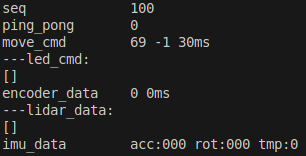
\includegraphics[width=0.5\textwidth, center]{img/Backend/print_wrapper_all.png}
    \caption{Python - Protobuf Konsolenausgabe}
    \label{fig:py_konsole_o}
\end{figure}

In Zukunft kann dies durch die Datenbank oder ein CSV Log abgelöst werden.
% 
Diese könnten automatisch nach Auffälligkeiten suchen 
und diese entsprechend melden und in einem Log abspeichern.

% \section{Protobuf Generierung}
% \initials{JS}
% % TODO
% Zurzeit nicht implementiert.

% Ein kleines Skript, welcher die Protobuff Dateien generiert
% und die Imports richtig setzt. 

% \section{Konfiguration Datei}
% \initials{JS}
% % TODO 
% Zurzeit nicht implementiert.

% Bestimmte Konfigurationen wie die Roboter Adressen 
% sollten in einer eigenen Konfigurations Datei landen und nicht im Code gesetzt sein.


\subsection{Optimierungsmöglichkeiten}
\initials{JS}
\label{subsec:Optimierungsmöglichkeiten}
\subsubsection{uvloop - schnellere Koroutinen}
\initials{JS}
% uvloop - drop in replacement
% https://github.com/MagicStack/uvloop
\texttt{uvloop} ist ein schneller Drop-in-Ersatz für den in \texttt{asyncio} integrierten Event-Loop.
% 
Dieser ist entsprechend in Cython entwickelt 
(Cython ist eigentlich Python, aber als Performanter C-Code kompiliert).
%
Ziel dieses Tausches ist es,
\texttt{asyncio} um einiges schneller zu machen, 
aber nicht von dem in \texttt{asyncio} gegebenen Verhalten abzuweichen.
% 
Als Drop-in-Ersatz geht dies so weit, 
dass die Abweichungen als Fehler kategorisiert werden.
%
In der Zukunft könnte der klassische \texttt{asyncio} Event-Loop mit
\texttt{uvloop} ausgetauscht werden,
falls dies notwendig wird.

\section{Test Codes}
\initials{JS}
Es wurde auch Testcode geschrieben, 
um die Kommunikationskanäle und Datenverarbeitung innerhalb 
und außerhalb des Backends zu testen.
% 
Insbesondere für die Fehlersuche ist Testcode eine gute Möglichkeit, 
um die Kommunikation und Datentausch zu testen.
%
Diese Testprogramme hat große Ähnlichkeiten mit der Kommunikation des tatsächlichen Backends, 
weshalb in diesem Abschnitt hauptsächlich auf deren Nutzen eingegangen.

\subsection{Einzelverbindung - Robot\_ws\_test.py}
\initials{JS}
Dieser Testcode ist verantwortlich, sich mit den Bots zu verbinden 
und dessen Daten zu lesen.
%
Er wurde mit einigen Konfigurationen erweitert und modifiziert 
und wird im Laufe des Projekts angepasst.

\subsection{Client und Server}
\initials{JS}
Dazu gehören \texttt{test\_wrap\_client.py} (als das Frontend) 
und \texttt{test\_wrap\_bot\_transceiver.py} (als die Bots).
%
Dies ist einfacher Code, welcher Client und Server (Bots und Server) simuliert, 
welche sich gegenseitig Protobuf-Pakete zuschicken. 
%
Dieser Code dient hauptsächlich dem Testen der Websocket-Kommunikation 
und auch zur Übung, wie Protobuf in Python zu verwenden ist.
% 
Die beiden Proramme senden und empfangen die Protobuf-Wrapper an das Backend,
welche die Pakete jeweils weiterleitet.
% 
Wenn ein Paket empfangen wird, wird dieses in die Konsole ausgegeben.
